\section{Trabalho e potencial eletrostático}

\frame{
	\frametitle{Trabalho da força elétrica}
	\begin{block}{Analogia mecânica}
		Trabalho e energia são grandezas diretamente proporcionais. Essa é a definição para o trabalho quando se estuda a energia mecânica.
		Vemos também na energia mecânica que o trabalho é realizado por uma força constante e paralela ao deslocamento de um corpo correspondente à variação de energia mecânica sofrida pelo corpo.
	\end{block}
}

\frame{
	\frametitle{Trabalho da força elétrica}
	\begin{block}{Definição}
		Consideremos o campo elétrico gerado por uma carga elétrica pontual $Q$, fixa num ponto $O$. Uma carga elétrica de prova $q$ é transportada do ponto $A$ para o ponto $B$ do campo, ao longo de uma linha de força. O trabalho $\tau_{A,B}$ realizado pela força elétrica, no deslocamento da carga elétrica $q$ do ponto A até o ponto $B$ é dado por: \\
		$$\boxed{\tau_{AB} = q \left( K \dfrac{Q}{d_A} - K \dfrac{Q}{d_B}\right) }$$
	\end{block}

	\centering
	

\tikzset{every picture/.style={line width=0.75pt}} %set default line width to 0.75pt        

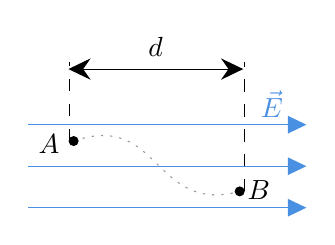
\begin{tikzpicture}[x=0.75pt,y=0.75pt,yscale=-1,xscale=1]
%uncomment if require: \path (0,300); %set diagram left start at 0, and has height of 300

%Curve Lines [id:da6177490068384819] 
\draw [color={rgb, 255:red, 155; green, 155; blue, 155 }  ,draw opacity=1 ] [dash pattern={on 0.84pt off 2.51pt}]  (137.88,127.88) .. controls (180,113.4) and (176,163.4) .. (217.88,152.13) ;


%Straight Lines [id:da7124330895115376] 
\draw [color={rgb, 255:red, 74; green, 144; blue, 226 }  ,draw opacity=1 ]   (116,120) -- (247,120) ;
\draw [shift={(250,120)}, rotate = 180] [fill={rgb, 255:red, 74; green, 144; blue, 226 }  ,fill opacity=1 ][line width=0.08]  [draw opacity=0] (8.93,-4.29) -- (0,0) -- (8.93,4.29) -- cycle    ;

%Straight Lines [id:da12792354611605283] 
\draw [color={rgb, 255:red, 74; green, 144; blue, 226 }  ,draw opacity=1 ]   (116,140) -- (247,140) ;
\draw [shift={(250,140)}, rotate = 180] [fill={rgb, 255:red, 74; green, 144; blue, 226 }  ,fill opacity=1 ][line width=0.08]  [draw opacity=0] (8.93,-4.29) -- (0,0) -- (8.93,4.29) -- cycle    ;

%Straight Lines [id:da4044562129660001] 
\draw [color={rgb, 255:red, 74; green, 144; blue, 226 }  ,draw opacity=1 ]   (116,160) -- (247,160) ;
\draw [shift={(250,160)}, rotate = 180] [fill={rgb, 255:red, 74; green, 144; blue, 226 }  ,fill opacity=1 ][line width=0.08]  [draw opacity=0] (8.93,-4.29) -- (0,0) -- (8.93,4.29) -- cycle    ;

%Shape: Circle [id:dp28224868607946574] 
\draw  [fill={rgb, 255:red, 0; green, 0; blue, 0 }  ,fill opacity=1 ] (135.75,127.88) .. controls (135.75,126.7) and (136.7,125.75) .. (137.88,125.75) .. controls (139.05,125.75) and (140,126.7) .. (140,127.88) .. controls (140,129.05) and (139.05,130) .. (137.88,130) .. controls (136.7,130) and (135.75,129.05) .. (135.75,127.88) -- cycle ;
%Shape: Circle [id:dp03942976292609046] 
\draw  [color={rgb, 255:red, 0; green, 0; blue, 0 }  ,draw opacity=1 ][fill={rgb, 255:red, 0; green, 0; blue, 0 }  ,fill opacity=1 ] (215.75,152.13) .. controls (215.75,150.95) and (216.7,150) .. (217.88,150) .. controls (219.05,150) and (220,150.95) .. (220,152.13) .. controls (220,153.3) and (219.05,154.25) .. (217.88,154.25) .. controls (216.7,154.25) and (215.75,153.3) .. (215.75,152.13) -- cycle ;
%Straight Lines [id:da5788684610773114] 
\draw  [dash pattern={on 4.5pt off 4.5pt}]  (135.75,127.88) -- (135.75,90) ;


%Straight Lines [id:da7063621547892809] 
\draw  [dash pattern={on 4.5pt off 4.5pt}]  (220,152.13) -- (220,90) ;


%Straight Lines [id:da8063380246624134] 
\draw    (138.35,93.2) -- (216.6,93.2) ;
\draw [shift={(219.6,93.2)}, rotate = 180] [fill={rgb, 255:red, 0; green, 0; blue, 0 }  ][line width=0.08]  [draw opacity=0] (10.72,-5.15) -- (0,0) -- (10.72,5.15) -- (7.12,0) -- cycle    ;
\draw [shift={(135.35,93.2)}, rotate = 0] [fill={rgb, 255:red, 0; green, 0; blue, 0 }  ][line width=0.08]  [draw opacity=0] (10.72,-5.15) -- (0,0) -- (10.72,5.15) -- (7.12,0) -- cycle    ;

% Text Node
\draw (233.4,110) node [color={rgb, 255:red, 74; green, 144; blue, 226 }  ,opacity=1 ]  {$\vec{E}$};
% Text Node
\draw (177.33,82.33) node   {$d$};
% Text Node
\draw (126,129.33) node   {$A$};
% Text Node
\draw (227.13,151.4) node   {$B$};


\end{tikzpicture}

%	\centerline{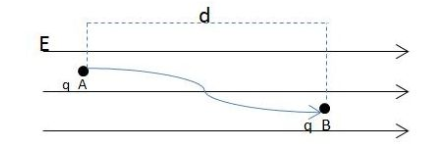
\includegraphics[width=0.6\linewidth]{Figuras/Ch09/trabalho1.PNG}}
}

\frame{
	\frametitle{Potencial elétrico no campo de uma carga pontual $Q$}
	\begin{block}{Motivação}
		Podemos dizer que o potencial elétrico é uma grandeza física que foi proposta a fim de descrever campos elétricos escalarmente. Portanto, podemos dizer que o conceito de potencial elétrico expressa o efeito de um campo elétrico em termos da posição dentro desse campo.
		\begin{itemize}
			\item Sendo uma \textbf{grandeza escalar}, necessita apenas, para ficar totalmente definida, da intensidade e de uma unidade de medida. Portanto, não requer nem direção, nem sentido.
		\end{itemize}
	\end{block}
}

\frame{
	\frametitle{Potencial elétrico no campo de uma carga pontual $Q$}
	\begin{block}{Fórmula}
		As grandezas $K \ \dfrac{Q}{d_A}$ e $K \ \dfrac{Q}{d_B}$ são chamados potenciais elétricos nos pontos $A$ e $B$ do campo elétrico gerado pela carga elétrica $Q$ e são indicadas, respectivamente por $V_A$ e $V_B$
		\begin{itemize}
			\item Quando $d_B$ tende a infinito, o trabalho tem seu valor máximo ($= V_A$)
		\end{itemize}
		$$\boxed{V = K \ \dfrac{Q}{d}}$$
	\end{block}
}

\frame{
	\frametitle{Potencial elétrico no campo de uma carga pontual $Q$}
	\begin{block}{Diferença de potencial}
		A diferença $V_A - V_B$ é indicada pela letra $U$ e é denominada \textbf{diferença de potencial} (d.d.p.) entre os pontos $A$ e $B$ ou \textbf{tensão elétrica} entre os pontos $A$ e $B$.
		\vspace{0.3cm}
		\begin{itemize}
			\item Da fórmula inicial de trabalho, temos:
		\end{itemize}
		$$\tau_{AB} = q \Bigg(K \ \dfrac{Q}{d_A} - K \ \dfrac{Q}{d_B}\Bigg) = q(V_A - V_B) \implies \boxed{\tau_{AB} = q \times U}$$
		\begin{itemize}
			\item A unidade de tensão pelo SI é o Joule por Coulomb (\si{\joule\per\coulomb}). A essa unidade convencionou-se dar o nome de \textbf{Volt} (\si{\volt}).
		\end{itemize}
	\end{block}
}

\frame{
	\frametitle{Potencial elétrico no campo de uma carga pontual $Q$}
	\begin{block}{Exemplo \#01}
		Uma carga pontual $Q = \SI{2.8e-5}{\coulomb}$ está colocada no vácuo. Considere um ponto $A$ distante de \SI{20}{\centi\meter} dessa carga, e outro ponto $B$ distante de \SI{30}{\centi\meter}. (a) Determine os potenciais elétricos nos pontos $A$ e $B$ e a d.d.p. entre eles. (b) Encontre o trabalho da força elétrica que age em uma carga de prova $q = \SI{2.0}{\nano\coulomb}$ ao ser deslocada de $A$ para $B$.
	\end{block}
}

\frame{
	\frametitle{Potencial elétrico no campo de uma carga pontual $Q$}
	\begin{block}{Resolução}
		(a)
		\begin{align*}
		V_A &= K \ \dfrac{Q}{d_A} = \num{9e9} \dfrac{\num{2.8e-5}}{\num{0,2}} = \SI{12.6e5}{\volt}\\
		V_B &= K \ \dfrac{Q}{d_B} = \num{9e9} \dfrac{\num{2.8e-5}}{\num{0,3}} = \SI{8.4e5}{\volt}
		\end{align*}
		Deste modo
		\[ U = V_A - V_B = \num{12.6e5} - \num{8.4e5} = \SI{4.2e5}{\volt} \]
		
		(b) $\tau_{A,B} = q \cdot U = \num{2e-9}\cdot \num{4,2e5} = \SI{8.4e-4}{\joule}$
	\end{block}
}

\frame{
	\frametitle{Potencial elétrico no campo de várias cargas}
	\begin{block}{Definição}
		Consideremos um campo elétrico que seja gerado por $n$ cargas puntiformes. Na região do campo, consideremos um ponto geométrico $P$, como mostra a figura. Qual o potencial elétrico resultante em $P$ e gerado pelas $n$ cargas elétricas?
	\end{block}

	\centering
	
	\setmyunit{1cm}
	
	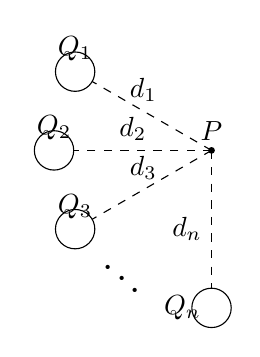
\begin{tikzpicture}
		\filldraw[black] (0,0) circle (1pt) node[above] {$ P $};
		
		\draw[dashed] (0,0) -- node[midway, above] {$ d_1 $} +(-30:-2);
		\draw[fill=white] (0,0) +(-30:-2) circle (0.25) node[above=0.25] {$ Q_1 $};
		
		\draw[dashed] (0,0) -- node[midway, above] {$ d_2 $} +(0:-2);
		\draw[fill=white] (0,0) +(0:-2) circle (0.25) node[above=0.25] {$ Q_2 $};
		
		\draw[dashed] (0,0) -- node[midway, above] {$ d_3 $} +(30:-2);
		\draw[fill=white] (0,0) +(30:-2) circle (0.25) node[above=0.25] {$ Q_3 $};
		
		\draw (0,0) +(55:-2) node[rotate=-40] {\Large $ \cdots $};
		
		\draw[dashed] (0,0) -- node[midway, left] {$ d_n $} +(90:-2);
		\draw[fill=white] (0,0) +(90:-2) circle (0.25) node[left=0.25] {$ Q_n $};
	\end{tikzpicture}
%	\centerline{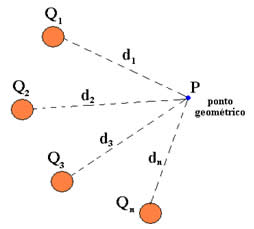
\includegraphics[width=0.45\linewidth]{Figuras/Ch09/potencial1.jpg}}
}

\frame{
	\frametitle{Potencial elétrico no campo de várias cargas}
	\begin{block}{Fórmula}
		Em primeiro lugar, deve-se calcular o potencial que cada carga cria \textbf{isoladamente} em $P$, usando a seguinte equação:
		$$V_1 = K \ \dfrac{Q_1}{d_1} \hspace{0.8cm} V_2 = K \ \dfrac{Q_2}{d_2} \hspace{0.8cm} ... \hspace{0.8cm} V_n = K \ \dfrac{Q_n}{d_n}$$
		Em seguida, \textbf{soma-se os potenciais obtidos}, levando em conta o sinal positivo ou negativo de cada um:
		$$\boxed{V = V_1 + V_2 + ... + V_n}$$
	\end{block}
}

\frame{
	\frametitle{Potencial elétrico no campo de várias cargas}
	\begin{block}{Exemplo \#01}
		Duas cargas pontuais $Q_1 = 2,0 \ \si{\micro}$C e $Q_2 = -4,0 \ \si{\micro}$C estão colocadas no vácuo a $90$ cm uma da outra. Determine o potencial no ponto médio da reta que une as duas cargas.
	\end{block}

	\begin{block}{Resolução}
		(a)
		\begin{align*}
			V_1 &= K \ \dfrac{Q_1}{d_1} = \num{9e9} \ \dfrac{\num{2.0e-6}}{\num{0,45}} = \SI{4.0e4}{\volt} \\
			V_2 &= K \ \dfrac{Q_2}{d_2} = \num{9e9} \ \dfrac{(\num{-4.0e-6})}{\num{0,45}} = \SI{-8.0e4}{\volt}
		\end{align*}
		Deste modo \[ V = V_1 + V_2 = \num{4.0e4} - \num{8.0e4} = \SI{-4.0e4}{\volt} \]
	\end{block}
}

\frame{
	\frametitle{Potencial elétrico no campo elétrico uniforme}
	\begin{block}{Definição}
		Considere uma carga elétrica positiva $q$ num ponto $A$ de um campo elétrico uniforme. A carga se desloca de $A$ para $B$ sob ação de uma força $F$ constante.
	\end{block}

	\centering
	
	\setmyunit{1cm}
	\begin{tikzpicture}
		\draw (0,0) rectangle (0.5,-4) (6,0) rectangle +(0.5,-4);
		
		\draw (2,-0.25) rectangle +(0.15,-0.15) node[pos=.5] {$ \cdot $};
		\draw (4,-0.25) rectangle +(0.15,-0.15) node[pos=.5] {$ \cdot $};
		
		\foreach \y in {0.25,0.75,...,3.75} {
			\draw (0.25,-\y) node {\Large $ + $};
			
			\draw[red,-Latex] (0.5,-\y) -- (6,-\y);
			
			\draw (6.25,-\y) node {\Large $ - $};
		}
	
		\draw[blue] (2,-0.15) node[above] {$ V_A $} -- (2,-3.85) (4,-0.15) node[above] {$ V_B $} -- (4,-3.85);
		\draw[dashed] (2,-3.85) -- +(0,-0.4) (4,-3.85) -- +(0,-0.4);
		
		\draw[<->] (2,-4.15) -- +(2,0) node[midway,above] {$ d $};
		
		\filldraw[fill=white] (2,-2) circle (0.25) node[] {$ q $};
		\draw[-Latex] ($ (2,-2)+(0.25,0) $) -- +(0.5,0);
		
		\draw[red] (5.5,-1) node {$ \vec{E} $};
	\end{tikzpicture}
%	\centerline{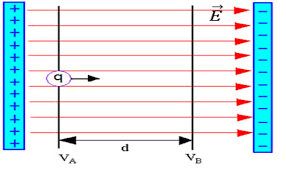
\includegraphics[width=0.7\linewidth]{Figuras/Ch09/uniforme.png}}
}

\frame{
	\frametitle{Potencial elétrico no campo elétrico uniforme}
	\begin{block}{Definição}
		Durante o deslocamento, a força elétrica realiza um trabalho $\tau_{AB}$, e como $F$ é constante, o trabalho pode ser calculado por: \\
		$$\tau_{AB} = F \times d$$ \\
		Porém, $F = q \times E$, então: \\
		$$\boxed{\tau_{AB} = q \times E \times d}$$ \\
		\vspace{0.3cm}
		Comparando com $\tau_{AB} = q \times U$, temos que $\boxed{U = E \times d}$, sendo $U = V_A - V_B$
	\end{block}
}

\frame{
	\frametitle{Potencial elétrico no campo elétrico uniforme}
	\begin{block}{Comportamento do potencial elétrico}
		De $E = U/d$, podemos verificar que a unidade de campo elétrico pode ser dada por \si{\volt\per\meter}. Verifica-se ainda, que o potencial em $A$ é maior que $B$. Isso significa que o potencial no campo elétrico uniforme \textbf{decresce} linearmente desde a placa positiva até a negativa.
	\end{block}

	\centering
	\setmyunit{1cm}
	\begin{tikzpicture}
		\draw[->,name path=Ox] (-0.5,0) -- (3,0) node[right] {$ d(\si{\meter}) $};
		\draw[->] (0,-1.5) -- (0,2) node[above] {$ v(\si{\volt}) $};
		
		\node[below left] at (0,0) {$ 0 $};
		
		\draw[name path=sl line] (0,1.5) -- (3,-1.5);
		
		\path[name path=pAx] (0,1) -- +(2,0);
		\path[name intersections={of=sl line and pAx, by=A}];
		
		\path[name path=pBx] (0,-1) -- +(3,0);
		\path[name intersections={of=sl line and pBx, by=B}];

		\draw[dashed] (0,1) node[left] {$ 20 $} -- (A) node[above right] {$ A $} -- (A|-0,0);
		
		\draw[dashed] (0,-1) node[left] {$ -20 $} -- (B) node[right] {$ B $} -- (B|-0,0);
		
	\end{tikzpicture}
%	\centerline{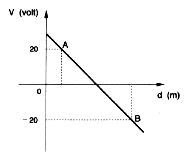
\includegraphics[width=0.45\linewidth]{Figuras/Ch09/uniforme2.jpg}}
}

\frame{
	\frametitle{Potencial elétrico no campo de um condutor esférico eletrizado}
	\begin{block}{Caso $\#$01: ponto $A$ interno}
		Como vimos anteriormente, a intensidade do vetor campo elétrico no interior de um condutor carregado de eletricidade e em equilíbrio eletrostático é sempre \textbf{nulo}.
		\begin{itemize}
			\item Assim, se colocarmos uma partícula eletrizada com carga $q$ sobre um ponto $A$ dentro da esfera e ela for deslocada para um ponto $B$, também interno à esfera, nenhum trabalho ($\tau_{AB}$) será realizado sobre ela e pela equação: $V_A - V_B = \tau_{AB}/q$, temos que $V_A = V_B$. \\

			\item Se $V_A$ fosse diferente de $V_B$ haveria fluxo de cargas entre esses dois pontos, e isso não pode ocorrer quando a esfera está em equilíbrio eletrostático. \\

			\item Dessa forma, podemos dizer que \textbf{no interior de uma esfera eletrizada em equilíbrio eletrostático, todos os pontos têm o mesmo potencial elétrico}.
		\end{itemize}
	\end{block}
}

\frame{
	\frametitle{Potencial elétrico no campo de um condutor esférico eletrizado}
	\begin{block}{Caso $\#$02: ponto $B$ pertencente à esfera}
		Quando temos um ponto $B$ exatamente na superfície da esfera ocorre novamente que o trabalho realizado para levar uma carga $q$ de $A$ até $B$ é igual a zero, dessa forma podemos concluir que \textbf{o potencial elétrico em qualquer ponto situado no interior de uma esfera eletrizada em equilíbrio eletrostático é igual ao potencial em sua superfície}.
		\begin{itemize}
			\item Devemos lembrar que esferas eletrizadas nessas condições de equilíbrio eletrostático podem ser consideradas como se tivessem toda sua carga concentrada em seu centro. \\
		\end{itemize}
		$$\boxed{V = K \ \dfrac{Q}{R}}$$
	\end{block}
}

\frame{
	\frametitle{Potencial elétrico no campo de um condutor esférico eletrizado}
	\begin{block}{Caso $\#$03: ponto $C$ externo}
		Se tivermos um ponto $C$ localizado externamente à esfera a uma distância $d$ do seu centro (dessa forma $d > R$), o potencial elétrico da esfera em $C$ pode ser calculado pela equação:
		$$\boxed{V = K \ \dfrac{Q}{d}}$$
	\end{block}
}

\frame{
	\frametitle{Potencial elétrico no campo de um condutor esférico eletrizado}
	\begin{block}{Resumindo...}
		O potencial para pontos no interior da esfera ($d \leq R$) é constante, e para pontos fora da esfera ($d > R$) decresce de forma inversamente proporcional à distância ($d$).
	\end{block}
	
	\setmyunit{1cm}
	
	\begin{minipage}{0.15\linewidth}
		\centering
		
		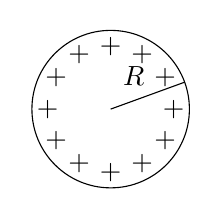
\begin{tikzpicture}
			\draw (0,0) circle (1);
			
			\draw (0,0) -- node[above,xshift=-5pt] {$ R $} (20:1);
			
			\foreach \x in {0,30,...,330}
				\draw (\x:0.8) node {$ + $};
		\end{tikzpicture}
	\end{minipage}
	\hfill
	\begin{minipage}{0.38\linewidth}
		\centering
		
		\begin{tikzpicture}[scale=0.5]
			\draw (-4,-3) rectangle (4,3); %CLP
		\draw (-4,0) -- (-2.5,0); %Div in out
		\draw (-2.5,-3) -- (-2.5,3); %Div cartoes
		\draw (-1.5,-2.5) rectangle (0,2.5); %Mem dados
		\draw (0.5,-2.5) rectangle (3.5,-1); %Mem prog
		\draw (1,0) rectangle (3,2); %CPU
		\draw (-4,-5) rectangle (4,-3); %Alimentacao
		\draw (-2.5,4) rectangle (4,6); %Term de prog
		
		\draw (1,2.6) node {CLP};
		
		\draw (-3.25,1.5) node[text width=1.5cm,align=center,rotate=90] {\small Cartões de input};
		
		\draw (-3.25,-1.5) node[text width=1.5cm,align=center,rotate=90] {\small Cartões de output};
		
		\node at (2,1) {\small CPU};
		
		\node[rotate=90,text width=1.5cm,align=center] at (-0.75,0) {\small Memória de dados};
		
		\node[text width=2cm,align=center] at (2,-1.75) {\footnotesize Memória de programa};
		
		\node at (-6,0) {Campo};
		
		\node at (0,-4) {Alimentação};
		
		\node[text width=3cm,align=center] at (0.75,5) {Terminal de programação};
		
		\draw[-Latex] (-8,1.5) -- node[above] {Entradas} +(4,0);
		\draw[Latex-] (-8,-1.5) -- node[below] {Saídas} +(4,0);
		\draw[-Latex] (-2.5,1.5) -- +(1,0);
		\draw[Latex-] (-2.5,-1.5) -- +(1,0);
		\draw[-Latex] (0,1.5) -- +(1,0);
		\draw[Latex-] (0,0.5) -- +(1,0);
		\draw[Latex-] (2,0) -- +(0,-1);
		
		\draw[-Latex] (-1.5,4) -- +(0,-1);
		\draw[Latex-] (3,4) -- +(0,-1);
	\end{tikzpicture}
	\end{minipage}
	\hfill
	\begin{minipage}{0.38\linewidth}
		\centering
		
		\newcommand{\innercolor}{gray!70!white}
	\newcommand{\outercolor}{gray!40!white}
	\newcommand{\leftcoil}{red!75!gray}
	\pgfmathsetmacro{\coilseparation}{0.02}
	
	\pgfmathsetmacro{\halflinewidth}{0.008}
	
	
	\begin{tikzpicture}[x={(\xx*1cm,\xy*1cm)},y={(\yx*1cm,\yy*1cm)},z={(\zx*1cm,\zy*1cm)}]
	\draw[\leftcoil, thick] (-0.02,5,1.125) -- +(0,2,0) (1.02,5,3.875) -- +(0,2,0);
	
	\draw[dashed,<->] ($ (-0.02,5,1.125)+(0,2,0) $) -- ($ (1.02,5,3.875)+(0,2,0) $);
	\node[rotate=85] at ($ (-0.02,5+2,1.125)!0.5!(1.02,5+2,3.875)+(0,0.2,0) $) {$ V_p $};
	
	\draw[-latex] (-0.02,6.5,1.325) -- node[above] {$ i_p $} +(0,-1,0);
	\draw[latex-] (1.02,0.02-0.5,1.3) -- node[above] {$ i_s $} +(0,-1,0);
	
	\filldraw[fill=\innercolor]  (0,1,1) -- (1,1,1) -- (1,4,1) -- (0,4,1) -- cycle;
	\filldraw[fill=\innercolor]  (1,4,1) -- (0,4,1) -- (0,4,4) -- (1,4,4) -- cycle;
	\filldraw[fill=\innercolor]  (0,0,0) -- (1,0,0) -- (1,0,5) -- (0,0,5) -- cycle;
	\filldraw[fill=\innercolor]  (0,0,5) -- (0,5,5) -- (1,5,5) -- (1,0,5) -- cycle;
	\filldraw[fill=\outercolor,even odd rule]    (0,0,0) -- (0,5,0) -- (0,5,5) -- (0,0,5) --cycle (0,1,1) -- (0,4,1) -- (0,4,4) -- (0,1,4) --cycle ;
	
	\begin{scope}
	\clip (0,3,1) -- (0,6,1) -- (0,6,4) -- (0,3,4);
	\foreach \z in {1.125,1.375,...,3.875}
	{   \draw[\leftcoil,thick] (0,5,\z) -- (-\coilseparation,5,\z) -- (-\coilseparation,4-\coilseparation,\z) -- (1+\coilseparation,4-\coilseparation,\z) -- (1+\coilseparation,4,\z);
	}
	\end{scope}
	
	
	\foreach \z in {1.25,1.75,...,3.75}
	{   \draw[blue,thick] (0,1,\z) -- (-\coilseparation,1,\z) -- (-\coilseparation,0-\coilseparation,\z) -- (1+\coilseparation,0-\coilseparation,\z) -- (1+\coilseparation,0,\z);
	}

	\draw[blue,thick] (1+\coilseparation,0+\coilseparation,1.1) -- +(0,-2,0) (-\coilseparation,1+\coilseparation,3.85) -- +(0,-3,0);
	
	\draw[dashed,<->] (1.02,-2+0.02,1.1) -- (-0.02,0.02-2,3.85);
	\node[rotate=-70] at ($ (1.02,-2+0.02,1.1)!0.5!(-0.02,0.02-2,3.85)+(0,-0.2,0) $) {$ V_s $};
	
	\draw[decorate,decoration={brace,amplitude=10pt},xshift=-4pt,yshift=0pt] (0,5,1.25) -- +(0,0,2.75);
	\draw[decorate,decoration={brace,amplitude=10pt},xshift=-4pt,yshift=0pt] (1.2,0,3.75) -- +(0,0,-2.6);
	\node[rotate=90] at (0,5.7,2.625) {$ N_p $ espiras};
	\node[rotate=-90] at (1.2,-0.5,2.5) {$ N_s $ espiras};
	
	\draw[dashed,postaction={decorate,decoration={markings,mark=between positions 0.1 and 1 step 0.2 with \arrow{Latex}}}] (0,4.5,0.5) -- (0,0.5,0.5) -- ++(0,0,4) -- ++(0,4,0) -- cycle;
	
	\draw[] (0,2.5,4.7)% -- +(0,-0.5,1.5)
	node[rotate=-10] {Fluxo magnético ($ \phi $)};
	
	\end{tikzpicture}
	\end{minipage}

%	\centerline{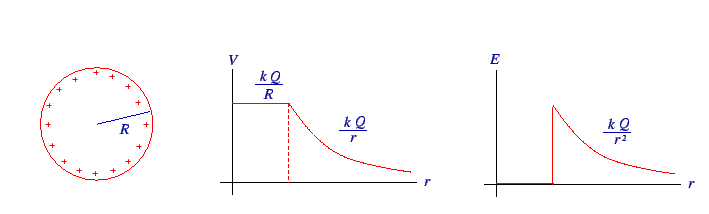
\includegraphics[width=1.1\linewidth]{Figuras/Ch09/potencialesfera.png}}
}

\section*{Exercícios}

\frame{
	\frametitle{Exercícios}
	\begin{block}{}

		01. Uma partícula eletrizada com carga $q = \SI{3.0}{\micro\coulomb}$ é colocada em repouso num ponto $A$ de um campo elétrico uniforme de intensidade $E = \SI{2.0e3}{\volt\per\meter}$, Num dado intervalo de tempo, ela se desloca para um ponto $B$. Sabendo que a d.d.p. entre os pontos $A$ e $B$ é $U = \SI{40}{\volt}$, determine: (a) o trabalho realizado pela força elétrica sobre a partícula; (b) a energia cinética da partícula ao atingir o ponto B; (c) o deslocamento realizado pela partícula; (d) a intensidade da força elétrica que age na partícula.

		\vspace{0.5cm}

		02. (FUVEST)  Uma esfera condutora de raio igual a \SI{1.6}{\centi\meter}, inicialmente neutra, tem massa igual a \SI{2.13225}{\gram} quando medida numa balança eletrônica digital de grande precisão. Supondo a esfera neutra, que quantidade de elétrons deve ser retirada desta esfera para que o potencial elétrico em seu interior seja de \SI{0.90}{\volt}?

	\end{block}
}


\section*{Referências}

\frame{
	\frametitle{Referências e Exercícios Complementares}
	\begin{itemize}
		\item Física, Ciência e Tecnologia – Vol 3. PENTEADO, Paulo César M; TORRES, Carlos Magno A. Ed. Moderna (2006)
	\end{itemize}
	%\centering{\alert{Página 36 - \textbf{1.6.1 até 1.6.5, 1.6.17 até 1.6.19}}} \\
	%https://www.youtube.com/watch?v=IUgS7Uw-qBI
	\centering{\alert{Lista de exercícios 09}}
}